

\section{Result tables} \label{sec:app_result_tables}




%  Generated from R function getRMSEResults: Get results from forecast simulation 
% -----------------------
% Get results from forecast simulation for the given location
% over a time range of 3 years, generate models in intervals of 1 week
% with 2,3 and 4 weeks of trainings data periods
% 4 locations are available from the forecast simulation (Application server):
%  1) Hamina, locationId 1, DA
%  2) St.Ghislain, locationId 2, DA
%  3) Portland, locationId 4, RT
%  4) Richmond, locationId 6, RT



\subsection{Results for Nord Pool Spot, FI (DA)} \label{ssec:app_tables_nord_pool_spot}



%> batchRMSEResults(1)
% latex table generated in R 3.1.1 by xtable 1.8-2 package
% Fri Mar 25 18:58:38 2016
\begin{table}[ht]
\centering
\begin{tabular}{rrrrrrrrrrr}
  \hline
 & 1h & 3h & 6h & 12h & 18h & 24h & 36h & 48h & 96h & 168h \\ 
  \hline
mean & 9.30 & 10.66 & 10.79 & 14.78 & 14.22 & 13.02 & 13.21 & 12.58 & 12.99 & 12.18 \\ 
  ses & 2.13 & 3.54 & 5.06 & 15.83 & 16.38 & 14.98 & 14.97 & 14.64 & 15.13 & 13.30 \\ 
  holts & 1.91 & 3.36 & 9.48 & 30.83 & 38.85 & 44.08 & 58.79 & 74.25 & 137.44 & 228.66 \\ 
  holtwinters & 3.22 & 7.15 & 13.18 & 26.22 & 36.32 & 46.07 & 65.31 & 85.66 & 167.14 & 289.51 \\ 
  arima & 2.11 & 3.08 & 4.65 & 13.66 & 13.89 & 12.67 & 12.87 & 12.61 & 13.68 & 12.98 \\ 
  tbats & 2.16 & 2.89 & 4.35 & 10.68 & 10.89 & 10.02 & 10.19 & 9.94 & 10.70 & 10.33 \\ 
   \hline
\end{tabular}
\caption{Forecast evaluation results based on RMSE for a trainings period of 2 weeks, Nord Pool Spot, Hamina}
\label{tab:app_results_hamina_2weeks}
\end{table}
% latex table generated in R 3.1.1 by xtable 1.8-2 package
% Fri Mar 25 18:58:38 2016
\begin{table}[ht]
\centering
\begin{tabular}{rrrrrrrrrrr}
  \hline
 & 1h & 3h & 6h & 12h & 18h & 24h & 36h & 48h & 96h & 168h \\ 
  \hline
mean & 9.40 & 10.75 & 10.90 & 15.03 & 14.46 & 13.25 & 13.44 & 12.81 & 13.27 & 12.42 \\ 
  ses & 2.14 & 3.56 & 5.06 & 15.84 & 16.38 & 14.98 & 14.97 & 14.63 & 15.14 & 13.31 \\ 
  holts & 1.91 & 3.38 & 9.51 & 30.88 & 38.90 & 44.15 & 58.90 & 74.39 & 137.77 & 229.23 \\ 
  holtwinters & 3.44 & 7.61 & 14.06 & 27.95 & 38.22 & 47.77 & 67.07 & 87.51 & 169.44 & 292.43 \\ 
  arima & 2.12 & 2.95 & 4.37 & 13.02 & 13.12 & 11.89 & 11.99 & 11.63 & 12.37 & 11.50 \\ 
  tbats & 2.15 & 3.04 & 4.73 & 11.23 & 11.41 & 10.51 & 10.57 & 10.33 & 11.05 & 10.67 \\ 
   \hline
\end{tabular}
\caption{Forecast evaluation results based on RMSE for a trainings period of 3 weeks, Nord Pool Spot, Hamina}
\label{tab:app_results_hamina_3weeks}
\end{table}
% latex table generated in R 3.1.1 by xtable 1.8-2 package
% Fri Mar 25 18:58:38 2016
\begin{table}[ht]
\centering
\begin{tabular}{rrrrrrrrrrr}
  \hline
 & 1h & 3h & 6h & 12h & 18h & 24h & 36h & 48h & 96h & 168h \\ 
  \hline
mean & 9.52 & 10.88 & 11.04 & 15.22 & 14.63 & 13.42 & 13.58 & 12.94 & 13.41 & 12.57 \\ 
  ses & 2.13 & 3.57 & 5.06 & 15.84 & 16.38 & 14.97 & 14.96 & 14.61 & 15.13 & 13.30 \\ 
  holts & 1.89 & 3.37 & 9.53 & 31.00 & 39.07 & 44.34 & 59.18 & 74.75 & 138.54 & 230.59 \\ 
  holtwinters & 5.58 & 11.05 & 17.33 & 33.52 & 44.92 & 54.87 & 76.25 & 98.63 & 189.26 & 327.09 \\ 
  arima & 1.98 & 2.85 & 4.39 & 12.69 & 12.79 & 11.60 & 11.73 & 11.35 & 12.06 & 11.12 \\ 
  tbats & 2.20 & 3.09 & 4.64 & 10.98 & 11.19 & 10.31 & 10.45 & 10.20 & 10.91 & 10.36 \\ 
   \hline
\end{tabular}
\caption{Forecast evaluation results based on RMSE for a trainings period of 4 weeks, Nord Pool Spot, Hamina}
\label{tab:app_results_hamina_4weeks}
\end{table}






\begin{landscape}

\subsection{Results for Belpex, BE (DA)} \label{ssec:app_tables_belpex}



%> batchRMSEResults(2)
% latex table generated in R 3.1.1 by xtable 1.8-2 package
% Fri Mar 25 18:58:51 2016
\begin{table}[ht]
\centering
\vspace*{-0.2in}
\begin{tabular}{rrrrrrrrrrr}
  \hline
 & 1h & 3h & 6h & 12h & 18h & 24h & 36h & 48h & 96h & 168h \\ 
  \hline
mean & 12.96 & 15.84 & 18.24 & 16.96 & 15.83 & 15.74 & 15.56 & 15.31 & 15.44 & 15.79 \\ 
  ses & 8.32 & 11.37 & 14.02 & 16.60 & 16.52 & 17.05 & 16.85 & 17.07 & 17.46 & 17.08 \\ 
  holts & 7.88 & 11.28 & 18.10 & 45.21 & 62.73 & 80.79 & 113.75 & 149.46 & 288.20 & 493.94 \\ 
  holtwinters & 10.77 & 21.02 & 34.17 & 61.39 & 86.76 & 113.05 & 164.22 & 216.22 & 424.16 & 736.39 \\ 
  arima & 6.86 & 7.10 & 7.82 & 14.34 & 15.42 & 15.41 & 15.64 & 16.11 & 17.79 & 18.47 \\ 
  tbats & 4.86E+49 & 1.05E+50 & 1.46E+50 & 1.45E+50 & 1.40E+50 & 1.39E+50 & 1.38E+50 & 1.37E+50 & 1.36E+50 & 1.35E+50 \\ 
   \hline
\end{tabular}
\caption{Forecast evaluation results based on RMSE for a trainings period of 2 weeks, Belpex, St.Ghislain}
\label{tab:app_results_stghislain_2weeks}
\end{table}
% latex table generated in R 3.1.1 by xtable 1.8-2 package
% Fri Mar 25 18:58:51 2016
\begin{table}[ht]
\centering
\vspace*{-0.1in}
\begin{tabular}{rrrrrrrrrrr}
  \hline
 & 1h & 3h & 6h & 12h & 18h & 24h & 36h & 48h & 96h & 168h \\ 
  \hline
mean & 13.27 & 16.10 & 18.41 & 17.27 & 16.18 & 16.06 & 15.90 & 15.66 & 15.75 & 16.07 \\ 
  ses & 8.37 & 11.41 & 14.07 & 16.64 & 16.56 & 17.08 & 16.88 & 17.10 & 17.50 & 17.10 \\ 
  holts & 7.80 & 11.29 & 18.07 & 45.41 & 63.10 & 81.37 & 114.61 & 150.60 & 290.39 & 497.90 \\ 
  holtwinters & 10.39 & 18.71 & 31.85 & 61.71 & 86.71 & 114.91 & 167.80 & 221.43 & 436.30 & 758.77 \\ 
  arima & 6.70 & 6.61 & 7.07 & 13.92 & 15.02 & 14.99 & 15.26 & 15.67 & 17.06 & 17.12 \\ 
  tbats & 6.05 & 6.50 & 7.12 & 11.95 & 13.17 & 13.40 & 13.71 & 14.11 & 14.98 & 15.05 \\ 
   \hline
\end{tabular}
\caption{Forecast evaluation results based on RMSE for a trainings period of 3 weeks, Belpex, St.Ghislain}
\label{tab:app_results_stghislain_3weeks}
\end{table}
% latex table generated in R 3.1.1 by xtable 1.8-2 package
% Fri Mar 25 18:58:51 2016
\begin{table}[hb]
\centering
%\vspace*{-0.4in}
\begin{tabular}{rrrrrrrrrrr}
  \hline
 & 1h & 3h & 6h & 12h & 18h & 24h & 36h & 48h & 96h & 168h \\ 
  \hline
mean & 13.62 & 16.34 & 18.54 & 17.44 & 16.36 & 16.22 & 16.07 & 15.82 & 15.89 & 16.19 \\ 
  ses & 8.38 & 11.45 & 14.12 & 16.68 & 16.59 & 17.11 & 16.91 & 17.12 & 17.52 & 17.12 \\ 
  holts & 7.82 & 11.30 & 18.05 & 45.14 & 62.69 & 80.72 & 113.69 & 149.35 & 287.92 & 493.58 \\ 
  holtwinters & 9.68 & 20.86 & 34.34 & 60.86 & 85.91 & 112.49 & 164.12 & 216.17 & 423.85 & 735.38 \\ 
  arima & 6.82 & 6.91 & 7.56 & 14.06 & 15.05 & 14.87 & 15.09 & 15.42 & 16.47 & 16.41 \\ 
  tbats & 2.53E+35 & 2.17E+36 & 3.83E+36 & 2.88E+36 & 3.16E+36 & 2.83E+36 & 2.73E+36 & 2.63E+36 & 2.36E+36 & 2.07E+36 \\ 
   \hline
\end{tabular}
\caption{Forecast evaluation results based on RMSE for a trainings period of 4 weeks, Belpex, St.Ghislain}
\label{tab:app_results_stghislain_4weeks}
\vspace*{-0.4in}
\end{table}



\subsection{Results for ISO New England, ME (RT)}


%> batchRMSEResults(4)
% latex table generated in R 3.1.1 by xtable 1.8-2 package
% Fri Mar 25 18:59:05 2016
\begin{table}[ht]
\centering
\vspace*{-0.2in}
\begin{tabular}{rrrrrrrrrrr}
  \hline
 & 1h & 3h & 6h & 12h & 18h & 24h & 36h & 48h & 96h & 168h \\ 
  \hline
mean & 19.21 & 21.35 & 22.93 & 24.24 & 28.47 & 28.56 & 27.93 & 29.36 & 30.92 & 31.17 \\ 
  ses & 7.92 & 10.71 & 12.94 & 21.12 & 27.62 & 28.38 & 28.25 & 30.32 & 33.99 & 34.90 \\ 
  holts & 16.74 & 26.25 & 42.47 & 84.48 & 120.17 & 149.95 & 210.04 & 274.13 & 527.63 & 906.49 \\ 
  holtwinters & 24.65 & 54.05 & 85.92 & 144.90 & 203.27 & 257.96 & 368.25 & 482.61 & 936.53 & 1615.73 \\ 
  arima & 9.78 & 13.81 & 16.13 & 20.09 & 25.98 & 26.87 & 27.18 & 29.37 & 34.24 & 37.68 \\ 
  tbats & 9.61E+16 & 5.92E+16 & 6.82E+16 & 7.15E+16 & 6.03E+16 & 5.48E+16 & 4.56E+16 & 3.97E+16 & 2.81E+16 & 2.13E+16 \\ 
   \hline
\end{tabular}
\caption{Forecast evaluation results based on RMSE for a trainings period of 2 weeks, ISO NE, Portland}
\label{tab:app_results_portland_2weeks}
\end{table}
% latex table generated in R 3.1.1 by xtable 1.8-2 package
% Fri Mar 25 18:59:05 2016
\begin{table}[ht]
\centering
\vspace*{-0.1in}
\begin{tabular}{rrrrrrrrrrr}
  \hline
 & 1h & 3h & 6h & 12h & 18h & 24h & 36h & 48h & 96h & 168h \\ 
  \hline
mean & 19.55 & 21.69 & 23.11 & 24.16 & 28.38 & 28.43 & 27.71 & 29.08 & 30.57 & 30.94 \\ 
  ses & 7.96 & 10.58 & 12.86 & 20.98 & 27.56 & 28.33 & 28.20 & 30.29 & 33.93 & 34.89 \\ 
  holts & 16.76 & 26.55 & 43.00 & 85.36 & 121.44 & 151.57 & 212.65 & 277.82 & 535.27 & 918.77 \\ 
  holtwinters & 22.72 & 53.73 & 107.68 & 218.76 & 311.85 & 412.94 & 605.67 & 801.89 & 1582.44 & 2751.86 \\ 
  arima & 9.42 & 13.01 & 15.81 & 19.23 & 24.53 & 25.21 & 25.17 & 26.90 & 30.67 & 32.61 \\ 
  tbats & 2.24E+18 & 2.61E+18 & 2.31E+18 & 1.98E+18 & 1.76E+18 & 1.58E+18 & 1.33E+18 & 1.16E+18 & 8.24E+17 & 6.23E+17 \\ 
   \hline
\end{tabular}
\caption{Forecast evaluation results based on RMSE for a trainings period of 3 weeks, ISO NE, Portland}
\label{tab:app_results_portland_3weeks}
\end{table}
% latex table generated in R 3.1.1 by xtable 1.8-2 package
% Fri Mar 25 18:59:05 2016
\begin{table}[ht]
\centering
\begin{tabular}{rrrrrrrrrrr}
  \hline
 & 1h & 3h & 6h & 12h & 18h & 24h & 36h & 48h & 96h & 168h \\ 
  \hline
mean & 19.92 & 22.05 & 23.52 & 24.76 & 28.95 & 28.83 & 28.13 & 29.56 & 31.07 & 31.61 \\ 
  ses & 7.70 & 10.26 & 12.61 & 20.76 & 27.36 & 28.11 & 27.95 & 30.07 & 33.72 & 34.67 \\ 
  holts & 16.47 & 27.14 & 45.95 & 93.96 & 134.70 & 169.48 & 239.48 & 313.17 & 603.78 & 1036.84 \\ 
  holtwinters & 18.60 & 43.70 & 79.50 & 139.59 & 204.63 & 265.58 & 386.07 & 508.92 & 999.22 & 1732.67 \\ 
  arima & 8.58 & 12.42 & 15.33 & 18.73 & 24.17 & 24.88 & 24.88 & 26.65 & 30.38 & 32.33 \\ 
  tbats & 3.55E+31 & 3.00E+32 & 2.59E+32 & 2.40E+32 & 2.34E+32 & 2.31E+32 & 2.27E+32 & 2.25E+32 & 2.18E+32 & 2.11E+32 \\ 
   \hline
\end{tabular}
\caption{Forecast evaluation results based on RMSE for a trainings period of 4 weeks, ISO NE, Portland}
\label{tab:app_results_portland_4weeks}
\vspace*{-0.4in}
\end{table}




\subsection{Results for PJM, VA (RT)}



%> batchRMSEResults(6)
% latex table generated in R 3.1.1 by xtable 1.8-2 package
% Fri Mar 25 18:59:07 2016
\begin{table}[ht]
\centering
\vspace*{-0.2in}
\begin{tabular}{rrrrrrrrrrr}
  \hline
 & 1h & 3h & 6h & 12h & 18h & 24h & 36h & 48h & 96h & 168h \\ 
  \hline
mean & 11.24 & 12.47 & 12.28 & 15.22 & 17.40 & 19.37 & 21.73 & 22.65 & 21.80 & 19.98 \\ 
  ses & 4.62 & 6.13 & 6.20 & 12.82 & 16.55 & 18.90 & 21.05 & 22.68 & 22.44 & 20.27 \\ 
  holts & 5.48 & 11.20 & 21.74 & 52.37 & 75.99 & 97.15 & 136.63 & 178.28 & 335.33 & 571.26 \\ 
  holtwinters & 13.35 & 34.52 & 60.06 & 110.03 & 155.78 & 204.00 & 297.67 & 388.74 & 757.00 & 1312.02 \\ 
  arima & 4.21 & 6.04 & 7.16 & 13.30 & 16.13 & 18.27 & 20.70 & 21.97 & 21.96 & 20.43 \\ 
  tbats & 4.88E+13 & 3.37E+13 & 6.17E+13 & 1.04E+14 & 1.01E+14 & 8.86E+13 & 8.59E+13 & 8.22E+13 & 7.72E+13 & 7.47E+13 \\ 
   \hline
\end{tabular}
\caption{Forecast evaluation results based on RMSE for a trainings period of 2 weeks, PJM, Richmond}
\label{tab:app_results_richmond_2weeks}
\end{table}
% latex table generated in R 3.1.1 by xtable 1.8-2 package
% Fri Mar 25 18:59:07 2016
\begin{table}[ht]
\centering
\vspace*{-0.1in}
\begin{tabular}{rrrrrrrrrrr}
  \hline
 & 1h & 3h & 6h & 12h & 18h & 24h & 36h & 48h & 96h & 168h \\ 
  \hline
mean & 11.31 & 12.54 & 12.31 & 15.20 & 17.37 & 19.32 & 21.65 & 22.54 & 21.58 & 19.77 \\ 
  ses & 4.70 & 6.19 & 6.26 & 12.87 & 16.58 & 18.95 & 21.12 & 22.77 & 22.50 & 20.32 \\ 
  holts & 5.74 & 11.54 & 22.09 & 52.45 & 75.77 & 96.79 & 136.06 & 177.31 & 333.00 & 566.99 \\ 
  holtwinters & 13.84 & 34.60 & 56.75 & 102.56 & 146.17 & 193.02 & 282.89 & 371.14 & 725.80 & 1259.30 \\ 
  arima & 3.78 & 5.49 & 6.12 & 12.00 & 15.03 & 17.35 & 19.89 & 21.26 & 21.09 & 19.36 \\ 
  tbats & 2.88 & 4.41 & 4.90 & 11.40 & 14.64 & 16.89 & 19.33 & 20.89 & 20.56 & 18.75 \\ 
   \hline
\end{tabular}
\caption{Forecast evaluation results based on RMSE for a trainings period of 3 weeks, PJM, Richmond}
\label{tab:app_results_richmond_3weeks}
\end{table}
% latex table generated in R 3.1.1 by xtable 1.8-2 package
% Fri Mar 25 18:59:07 2016
\begin{table}[ht]
\centering
\begin{tabular}{rrrrrrrrrrr}
  \hline
 & 1h & 3h & 6h & 12h & 18h & 24h & 36h & 48h & 96h & 168h \\ 
  \hline
mean & 11.34 & 12.56 & 12.32 & 15.08 & 17.25 & 19.24 & 21.64 & 22.55 & 21.64 & 19.82 \\ 
  ses & 4.73 & 6.25 & 6.29 & 12.90 & 16.62 & 19.01 & 21.20 & 22.86 & 22.59 & 20.42 \\ 
  holts & 5.70 & 11.42 & 22.02 & 52.42 & 76.01 & 97.17 & 136.67 & 178.24 & 335.44 & 571.65 \\ 
  holtwinters & 14.30 & 37.76 & 64.13 & 116.26 & 166.12 & 219.01 & 319.68 & 418.22 & 813.04 & 1409.65 \\ 
  arima & 3.70 & 5.44 & 6.04 & 12.09 & 15.08 & 17.30 & 19.88 & 21.16 & 21.03 & 19.39 \\ 
  tbats & 5.83E+55 & 2.82E+99 & 1.36E+109 & 9.65E+108 & 7.88E+108 & 6.82E+108 & 5.57E+108 & 4.82E+108 & 3.41E+108 & 2.58E+108 \\ 
   \hline
\end{tabular}
\caption{Forecast evaluation results based on RMSE for a trainings period of 4 weeks, PJM, Richmond}
\label{tab:app_results_richmond_4weeks}
\vspace*{-0.4in}
\end{table}

\end{landscape}






\section{Result graphs} \label{sec:app_result_graphs}

\FloatBarrier
\subsection{Results for Nord Pool Spot, FI (DA)} \label{ssec:app_graphs_nord_pool_spot}


\begin{figure}[!ht]
	\centering
		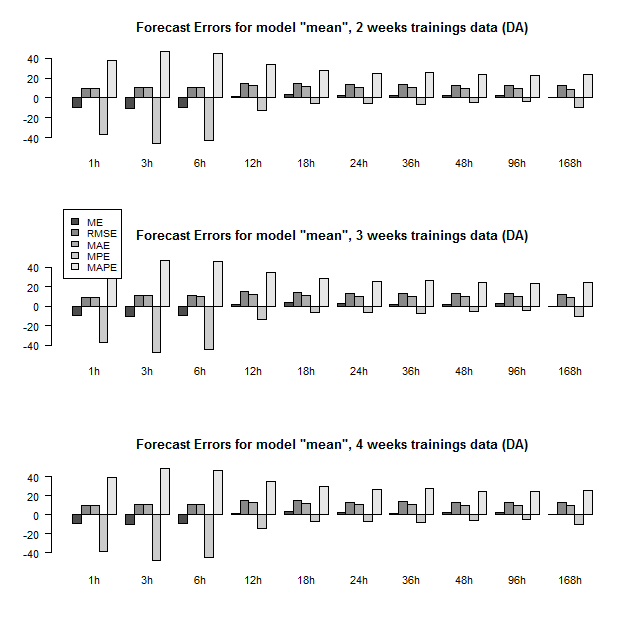
\includegraphics[width=0.85\textwidth]{figures/appendix_forecast_results/da_sim_1_x_1w_1w_mean.png}
	\caption{Aggregated accuracy measures for Mean model and trainings data of 2, 3 and 4 weeks, Nord
Pool Spot, Hamina}
	\label{fig:app_da_sim_1_x_1w_1w_mean}
\end{figure}



\begin{figure}[!ht]
	\centering
	\vspace*{-1.2in}
		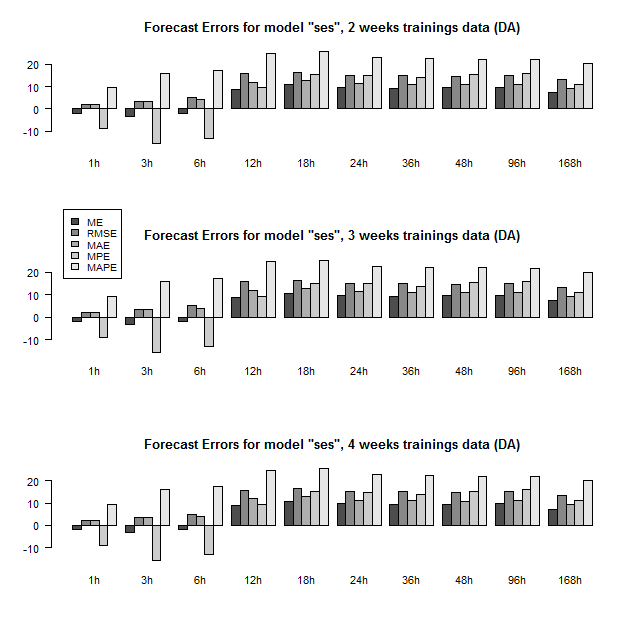
\includegraphics[width=0.85\textwidth]{figures/appendix_forecast_results/da_sim_1_x_1w_1w_ses.png}
	\caption{Aggregated accuracy measures for SES model and trainings data of 2, 3 and 4 weeks, Nord
Pool Spot, Hamina}
	\label{fig:app_da_sim_1_x_1w_1w_ses}
\end{figure}

\begin{figure}[!ht]
	\centering
		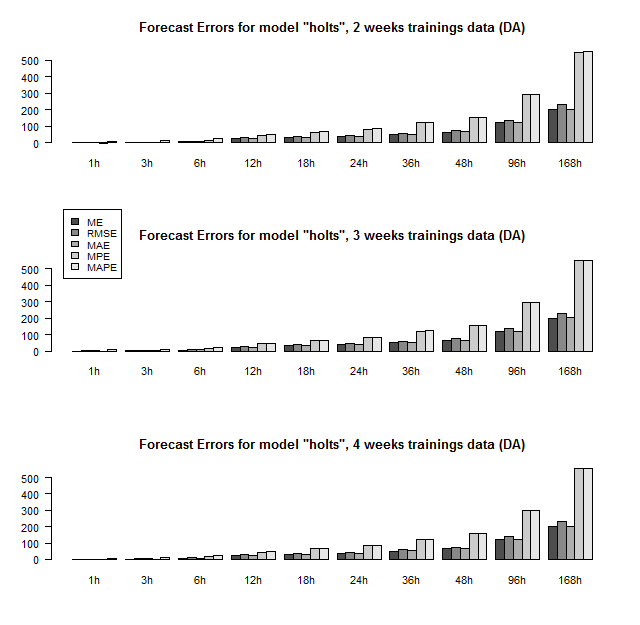
\includegraphics[width=0.85\textwidth]{figures/appendix_forecast_results/da_sim_1_x_1w_1w_holts.png}
	\caption{Aggregated accuracy measures for Holts model and trainings data of 2, 3 and 4 weeks, Nord
Pool Spot, Hamina}
	\label{fig:app_da_sim_1_x_1w_1w_holts}
	\vspace*{-1.6in}
\end{figure}




\begin{figure}[!ht]
	\centering
	\vspace*{-1.2in}
		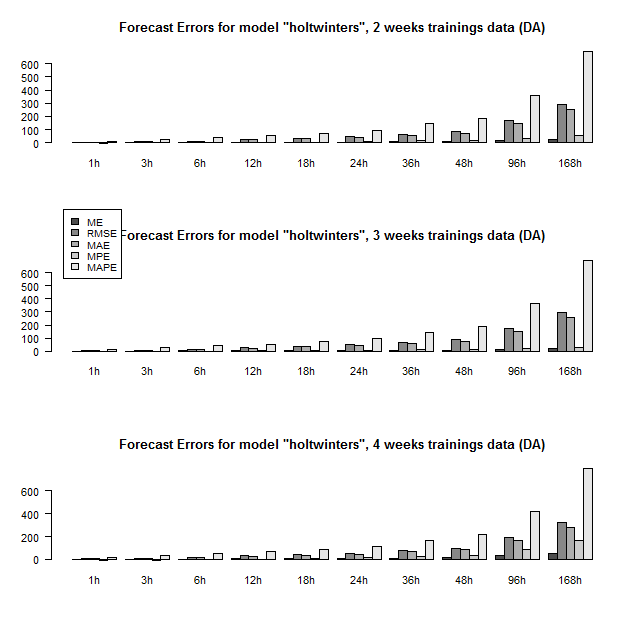
\includegraphics[width=0.85\textwidth]{figures/appendix_forecast_results/da_sim_1_x_1w_1w_holtwinters.png}
	\caption{Aggregated accuracy measures for HoltWinters model and trainings data of 2, 3 and 4 weeks, Nord
Pool Spot, Hamina}
	\label{fig:app_da_sim_1_x_1w_1w_holtwinters}
\end{figure}

\begin{figure}[!ht]
	\centering
		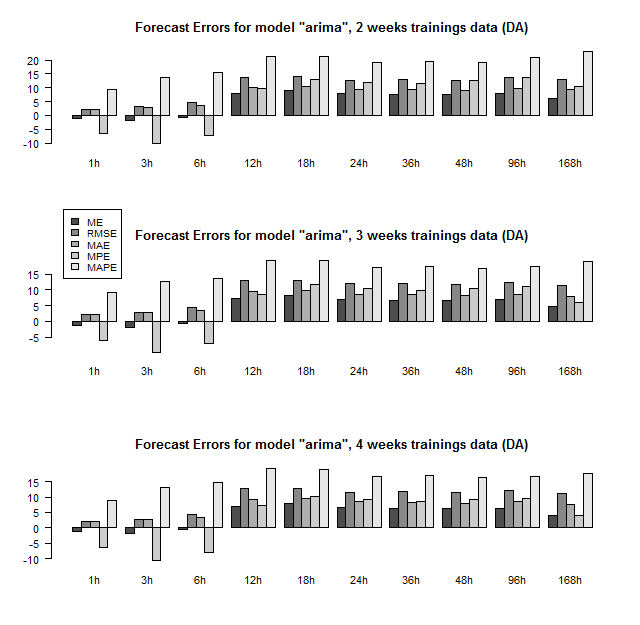
\includegraphics[width=0.85\textwidth]{figures/appendix_forecast_results/da_sim_1_x_1w_1w_arima.png}
	\caption{Aggregated accuracy measures for ARIMA model and trainings data of 2, 3 and 4 weeks, Nord
Pool Spot, Hamina}
	\label{fig:app_da_sim_1_x_1w_1w_arima}
	\vspace*{-1.6in}
\end{figure}




\begin{figure}[!ht]
	\centering
		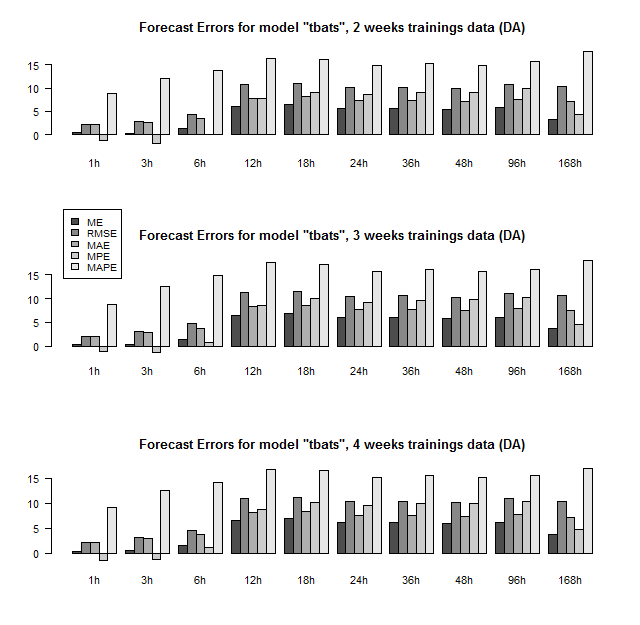
\includegraphics[width=0.85\textwidth]{figures/appendix_forecast_results/da_sim_1_x_1w_1w_tbats.png}
	\caption{Aggregated accuracy measures for TBATS model and trainings data of 2, 3 and 4 weeks, Nord
Pool Spot, Hamina}
	\label{fig:app_da_sim_1_x_1w_1w_tbats}
\end{figure}



\FloatBarrier
\subsection{Results for Belpex, BE (DA)} \label{ssec:app_graphs_belpex}


\begin{figure}[!ht]
	\centering
		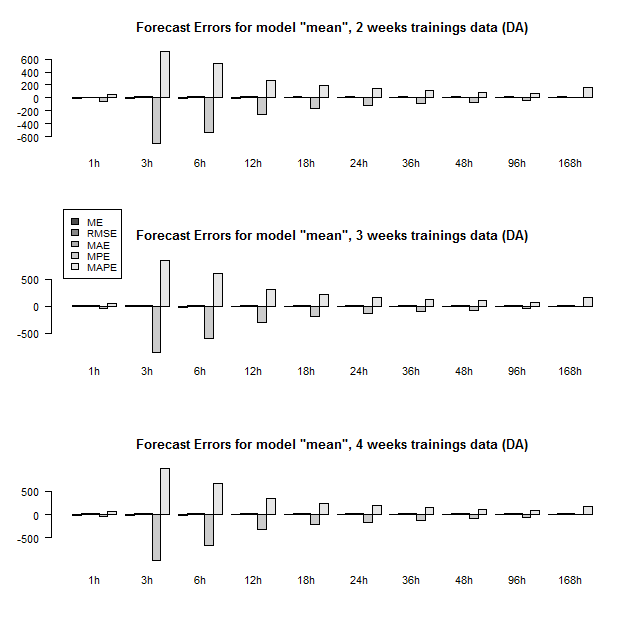
\includegraphics[width=0.85\textwidth]{figures/appendix_forecast_results/da_sim_2_x_1w_1w_mean.png}
	\caption{Aggregated accuracy measures for Mean model and trainings data of 2, 3 and 4 weeks, Belpex, St.Ghislain}
	\label{fig:app_da_sim_2_x_1w_1w_mean}
\end{figure}



\begin{figure}[!ht]
	\centering
	\vspace*{-1.2in}
		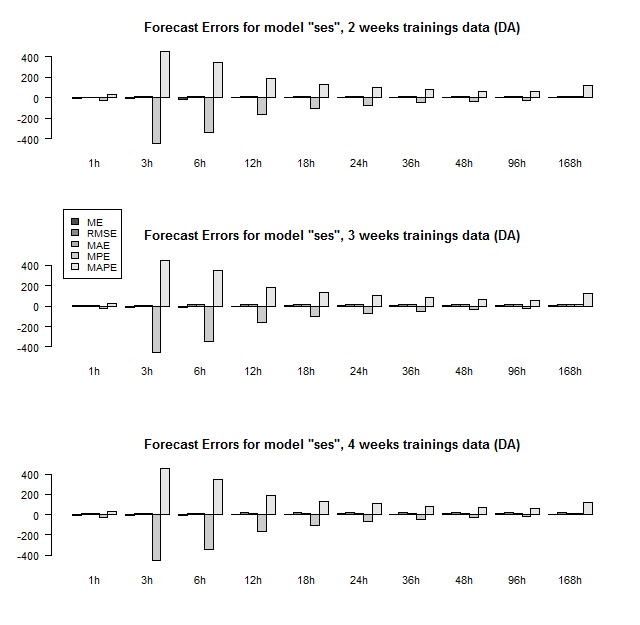
\includegraphics[width=0.85\textwidth]{figures/appendix_forecast_results/da_sim_2_x_1w_1w_ses.png}
	\caption{Aggregated accuracy measures for SES model and trainings data of 2, 3 and 4 weeks, Belpex, St.Ghislain}
	\label{fig:app_da_sim_2_x_1w_1w_ses}
\end{figure}

\begin{figure}[!ht]
	\centering
		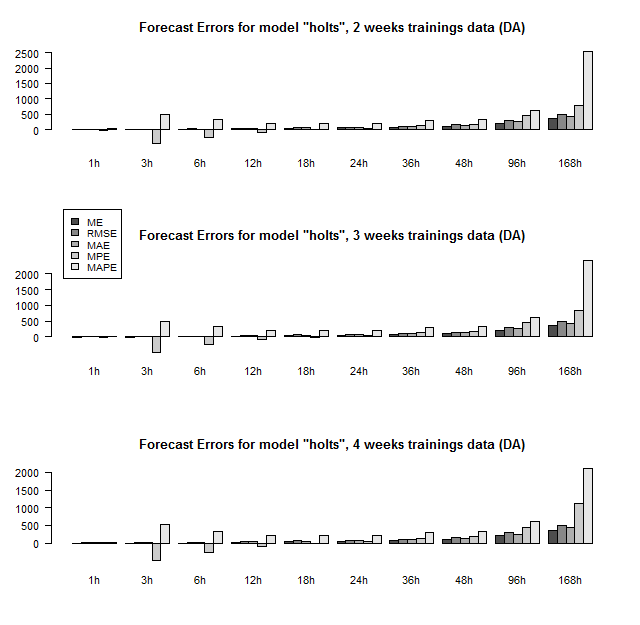
\includegraphics[width=0.85\textwidth]{figures/appendix_forecast_results/da_sim_2_x_1w_1w_holts.png}
	\caption{Aggregated accuracy measures for Holts model and trainings data of 2, 3 and 4 weeks, Belpex, St.Ghislain}
	\label{fig:app_da_sim_2_x_1w_1w_holts}
	\vspace*{-1.6in}
\end{figure}




\begin{figure}[!ht]
	\centering
	\vspace*{-1.2in}
		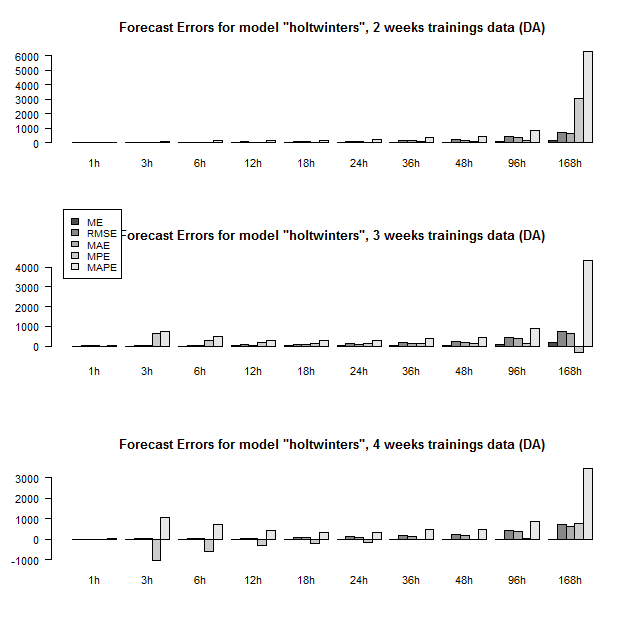
\includegraphics[width=0.85\textwidth]{figures/appendix_forecast_results/da_sim_2_x_1w_1w_holtwinters.png}
	\caption{Aggregated accuracy measures for HoltWinters model and trainings data of 2, 3 and 4 weeks, Belpex, St.Ghislain}
	\label{fig:app_da_sim_2_x_1w_1w_holtwinters}
\end{figure}

\begin{figure}[!ht]
	\centering
		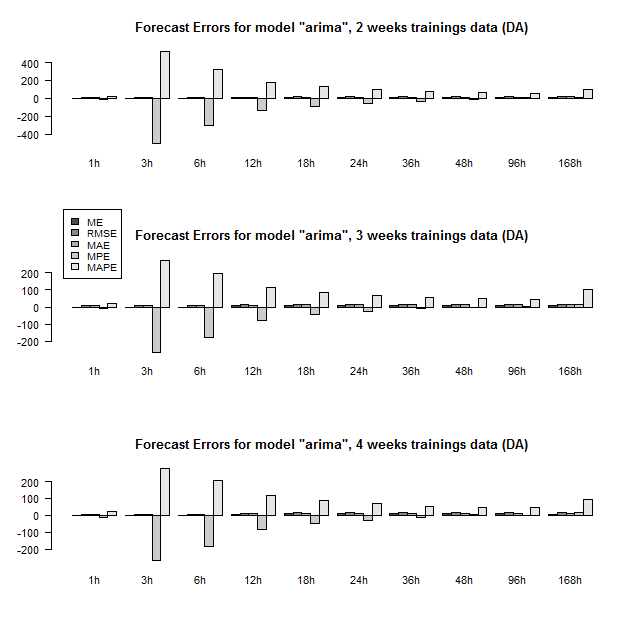
\includegraphics[width=0.85\textwidth]{figures/appendix_forecast_results/da_sim_2_x_1w_1w_arima.png}
	\caption{Aggregated accuracy measures for ARIMA model and trainings data of 2, 3 and 4 weeks, Belpex, St.Ghislain}
	\label{fig:app_da_sim_2_x_1w_1w_arima}
	\vspace*{-1.6in}
\end{figure}




\begin{figure}[!ht]
	\centering
		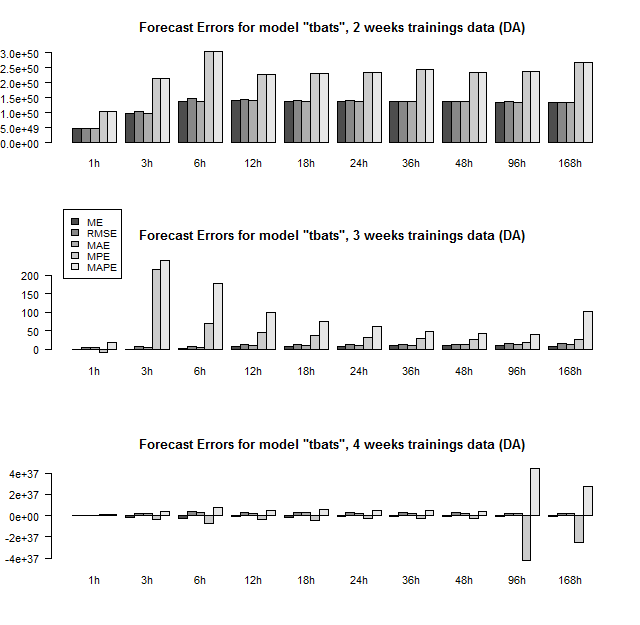
\includegraphics[width=0.85\textwidth]{figures/appendix_forecast_results/da_sim_2_x_1w_1w_tbats.png}
	\caption{Aggregated accuracy measures for TBATS model and trainings data of 2, 3 and 4 weeks, Belpex, St.Ghislain}
	\label{fig:app_da_sim_2_x_1w_1w_tbats}
\end{figure}




\FloatBarrier
\subsection{Results for ISO New England, ME (RT)}




\begin{figure}[!ht]
	\centering
		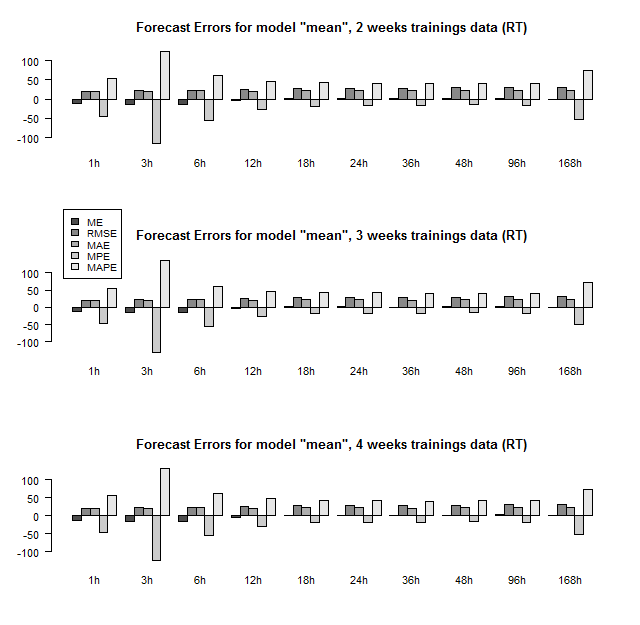
\includegraphics[width=0.85\textwidth]{figures/appendix_forecast_results/rt_sim_4_x_1w_1w_mean.png}
	\caption{Aggregated accuracy measures for Mean model and trainings data of 2, 3 and 4 weeks, ISO NE, Portland}
	\label{fig:app_rt_sim_4_x_1w_1w_mean}
\end{figure}



\begin{figure}[!ht]
	\centering
	\vspace*{-1.2in}
		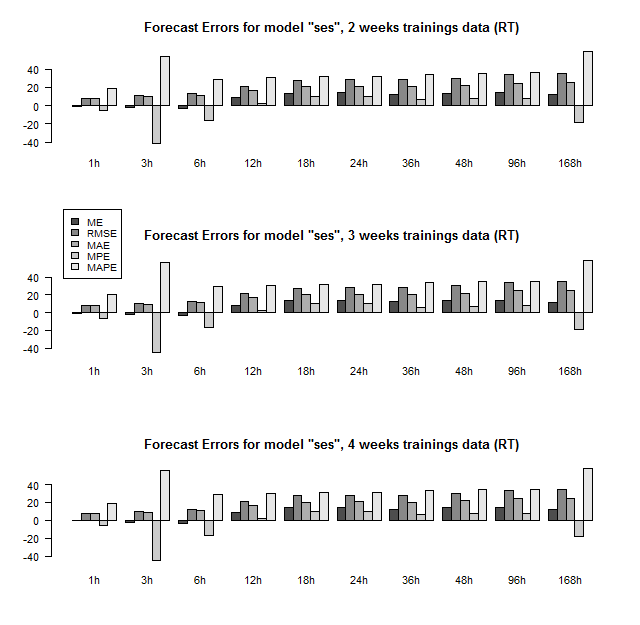
\includegraphics[width=0.85\textwidth]{figures/appendix_forecast_results/rt_sim_4_x_1w_1w_ses.png}
	\caption{Aggregated accuracy measures for SES model and trainings data of 2, 3 and 4 weeks, ISO NE, Portland}
	\label{fig:app_rt_sim_4_x_1w_1w_ses}
\end{figure}

\begin{figure}[!ht]
	\centering
		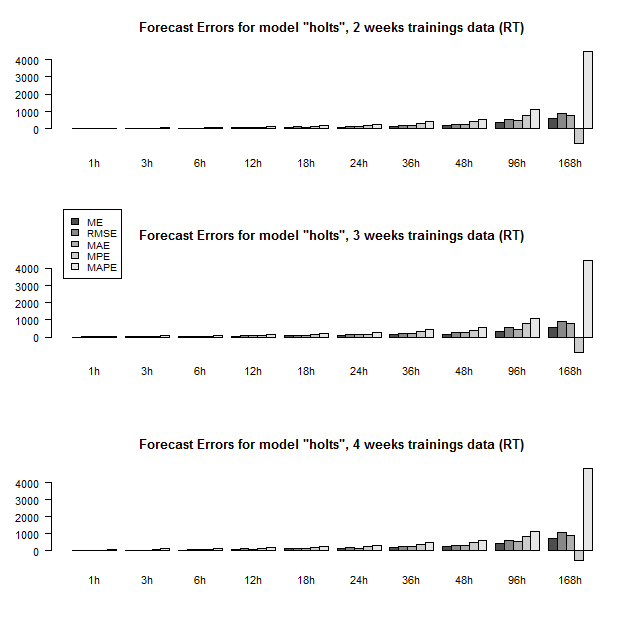
\includegraphics[width=0.85\textwidth]{figures/appendix_forecast_results/rt_sim_4_x_1w_1w_holts.png}
	\caption{Aggregated accuracy measures for Holts model and trainings data of 2, 3 and 4 weeks, ISO NE, Portland}
	\label{fig:app_rt_sim_4_x_1w_1w_holts}
	\vspace*{-1.6in}
\end{figure}




\begin{figure}[!ht]
	\centering
	\vspace*{-1.2in}
		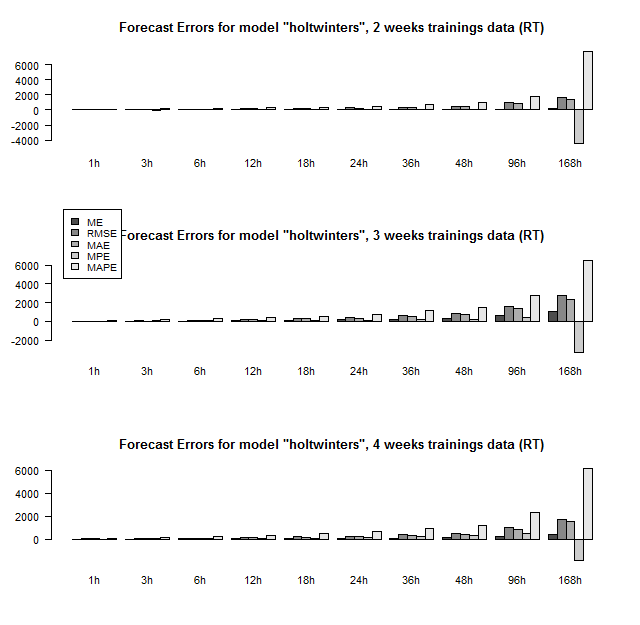
\includegraphics[width=0.85\textwidth]{figures/appendix_forecast_results/rt_sim_4_x_1w_1w_holtwinters.png}
	\caption{Aggregated accuracy measures for HoltWinters model and trainings data of 2, 3 and 4 weeks, ISO NE, Portland}
	\label{fig:app_rt_sim_4_x_1w_1w_holtwinters}
\end{figure}

\begin{figure}[!ht]
	\centering
		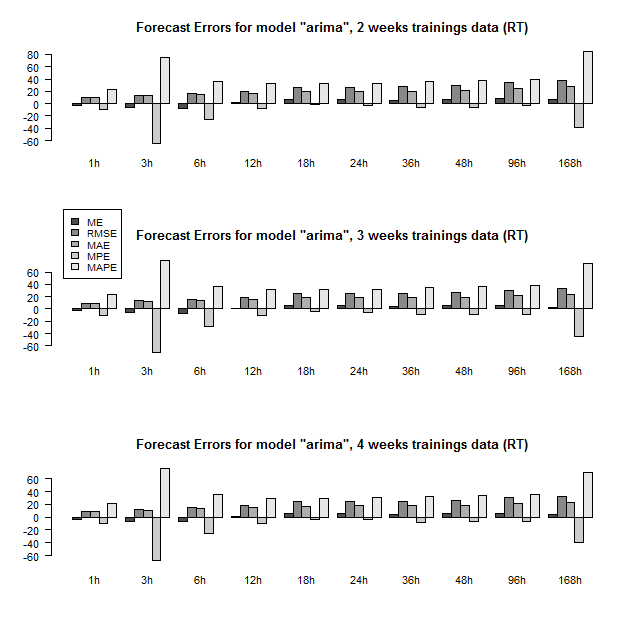
\includegraphics[width=0.85\textwidth]{figures/appendix_forecast_results/rt_sim_4_x_1w_1w_arima.png}
	\caption{Aggregated accuracy measures for ARIMA model and trainings data of 2, 3 and 4 weeks, ISO NE, Portland}
	\label{fig:app_rt_sim_4_x_1w_1w_arima}
	\vspace*{-1.6in}
\end{figure}




\begin{figure}[!ht]
	\centering
		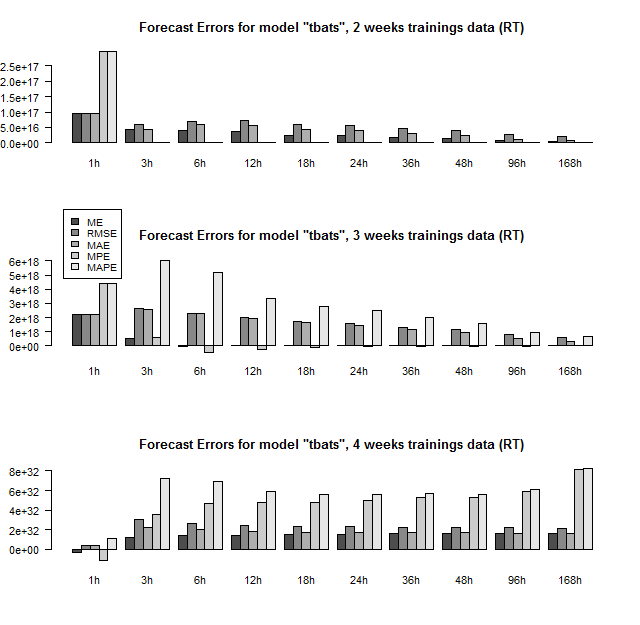
\includegraphics[width=0.85\textwidth]{figures/appendix_forecast_results/rt_sim_4_x_1w_1w_tbats.png}
	\caption{Aggregated accuracy measures for TBATS model and trainings data of 2, 3 and 4 weeks, ISO NE, Portland}
	\label{fig:app_rt_sim_4_x_1w_1w_tbats}
\end{figure}



\FloatBarrier
\subsection{Results for PJM, VA (RT)}



\begin{figure}[!ht]
	\centering
		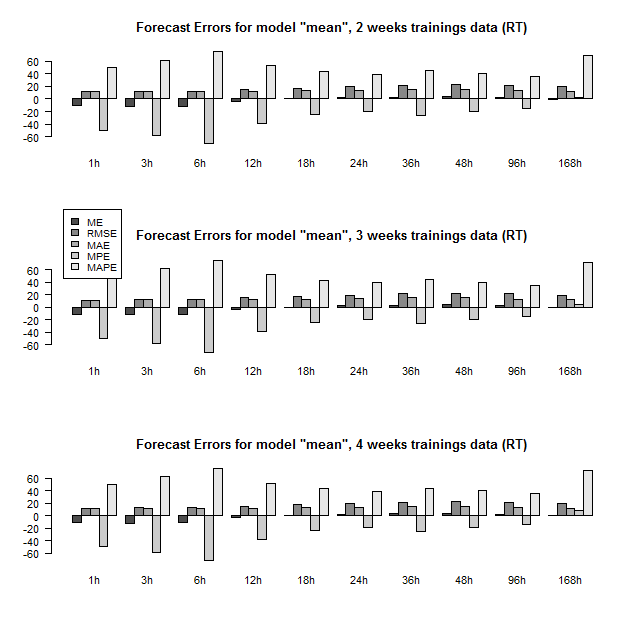
\includegraphics[width=0.85\textwidth]{figures/appendix_forecast_results/rt_sim_6_x_1w_1w_mean.png}
	\caption{Aggregated accuracy measures for Mean model and trainings data of 2, 3 and 4 weeks, PJM, Richmond}
	\label{fig:app_rt_sim_6_x_1w_1w_mean}
\end{figure}



\begin{figure}[!ht]
	\centering
	\vspace*{-1.2in}
		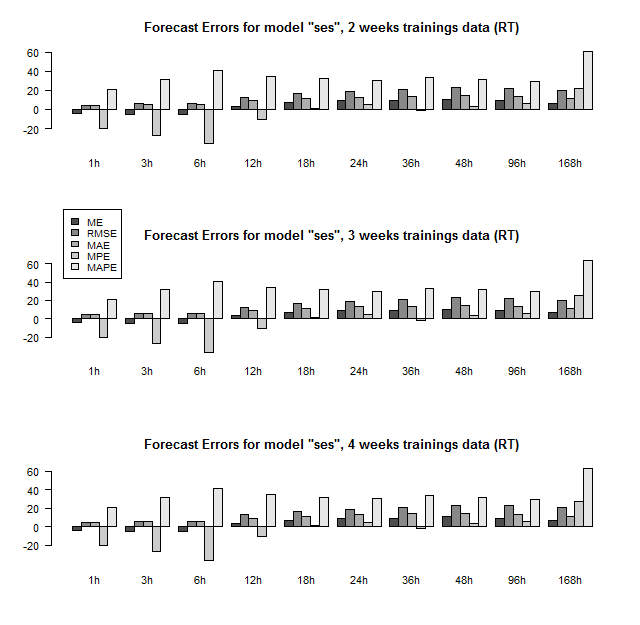
\includegraphics[width=0.85\textwidth]{figures/appendix_forecast_results/rt_sim_6_x_1w_1w_ses.png}
	\caption{Aggregated accuracy measures for SES model and trainings data of 2, 3 and 4 weeks, PJM, Richmond}
	\label{fig:app_rt_sim_6_x_1w_1w_ses}
\end{figure}

\begin{figure}[!ht]
	\centering
		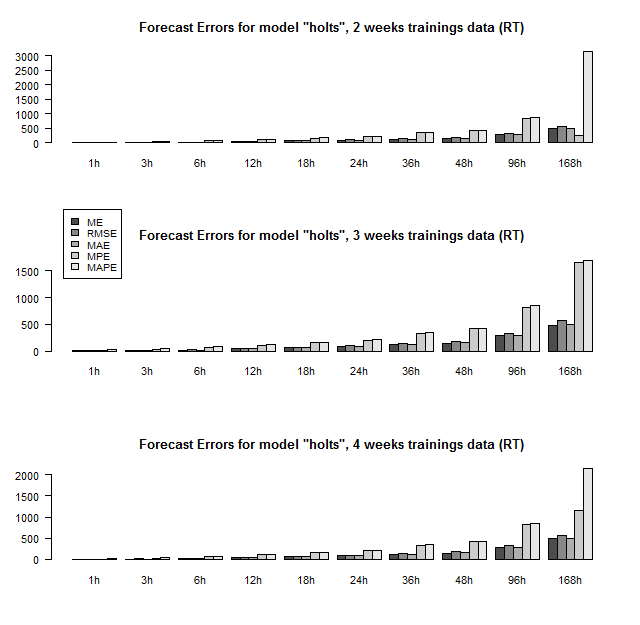
\includegraphics[width=0.85\textwidth]{figures/appendix_forecast_results/rt_sim_6_x_1w_1w_holts.png}
	\caption{Aggregated accuracy measures for Holts model and trainings data of 2, 3 and 4 weeks, PJM, Richmond}
	\label{fig:app_rt_sim_6_x_1w_1w_holts}
	\vspace*{-1.6in}
\end{figure}




\begin{figure}[!ht]
	\centering
	\vspace*{-1.2in}
		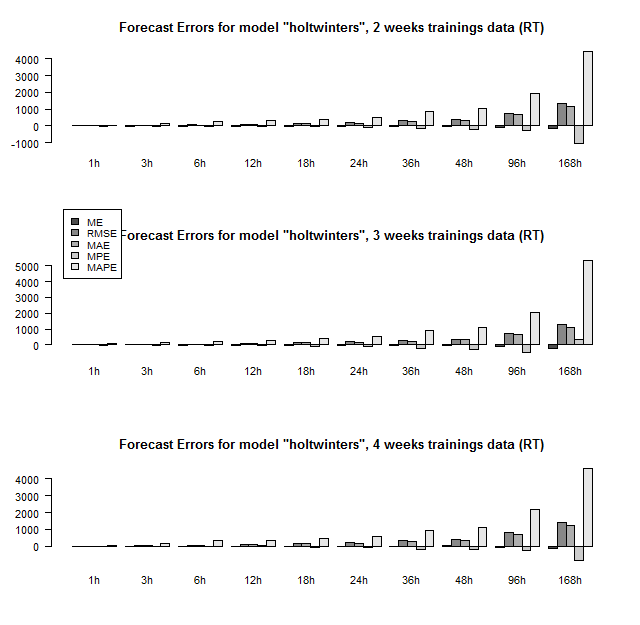
\includegraphics[width=0.85\textwidth]{figures/appendix_forecast_results/rt_sim_6_x_1w_1w_holtwinters.png}
	\caption{Aggregated accuracy measures for HoltWinters model and trainings data of 2, 3 and 4 weeks, PJM, Richmond}
	\label{fig:app_rt_sim_6_x_1w_1w_holtwinters}
\end{figure}

\begin{figure}[!ht]
	\centering
		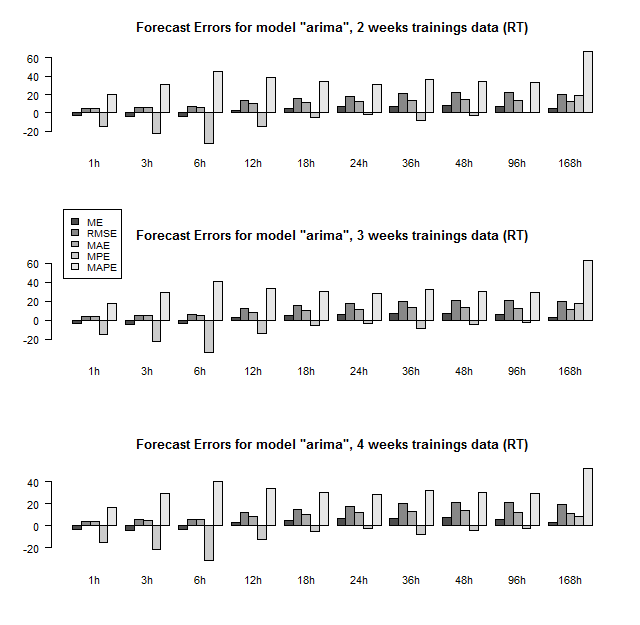
\includegraphics[width=0.85\textwidth]{figures/appendix_forecast_results/rt_sim_6_x_1w_1w_arima.png}
	\caption{Aggregated accuracy measures for ARIMA model and trainings data of 2, 3 and 4 weeks, PJM, Richmond}
	\label{fig:app_rt_sim_6_x_1w_1w_arima}
	\vspace*{-1.6in}
\end{figure}




\begin{figure}[!ht]
	\centering
		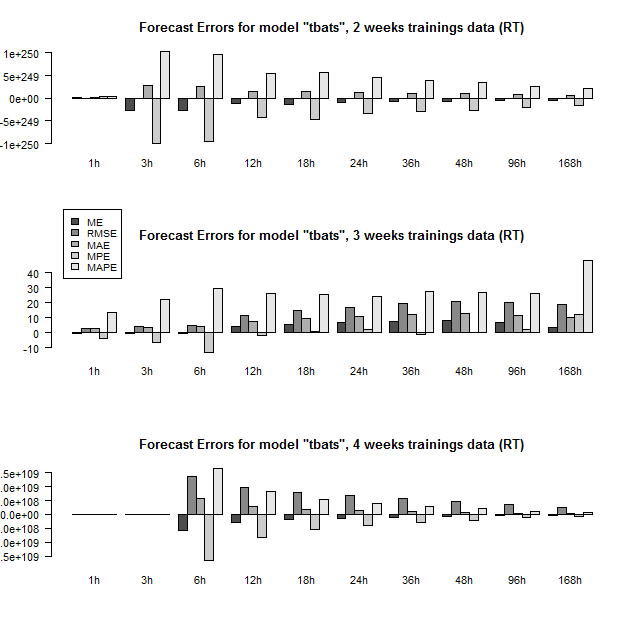
\includegraphics[width=0.85\textwidth]{figures/appendix_forecast_results/rt_sim_6_x_1w_1w_tbats.png}
	\caption{Aggregated accuracy measures for TBATS model and trainings data of 2, 3 and 4 weeks, PJM, Richmond}
	\label{fig:app_rt_sim_6_x_1w_1w_tbats}
\end{figure}

